\section{Our Approach}
\subsection{Stages}
\begin{frame}
\begin{itemize}
  \frametitle{Stages of Project Development}

  \item Identify program equivalency (correctness) properties:
  \begin{itemize}
    \item Initially just functional equivalence?
  \end{itemize}

  \item Identify Pig programs over which we will write proofs:
  \begin{itemize}
    \item Programs with limited data types?
    \item Programs without user defined functions (UDFs)?
    \item Programs with some subset of UDFs?
    \item All well-typed programs?
  \end{itemize}

  \item Implement all of this in Coq:
  \begin{itemize}
    \item Two languages.
    \item Two semantic models.
    \item Existing compilation algo.
    \item Prove correctness/equivalency w.r.t. this compilation algo.
  \end{itemize}

\end{itemize}
\end{frame}

\subsection{Operational Semantics}
\begin{frame}
  \frametitle{Concurrency in Operational Semantics}
  We expect that Pig should be able to modeled with sequential or non-concurrent
  semantics.

  However, MapReduce should be modeled with concurrent semantics.
\end{frame}

\begin{frame}
  \frametitle{Concern}
  Our correctness proofs should be performed over all (admissible) concurrent
  executions and w.r.t. a parameterized number of mappers and reducers.
\end{frame}

\begin{frame}
  \frametitle{Nondeterministic MapReduce Operational Semantics}
  \begin{figure}
    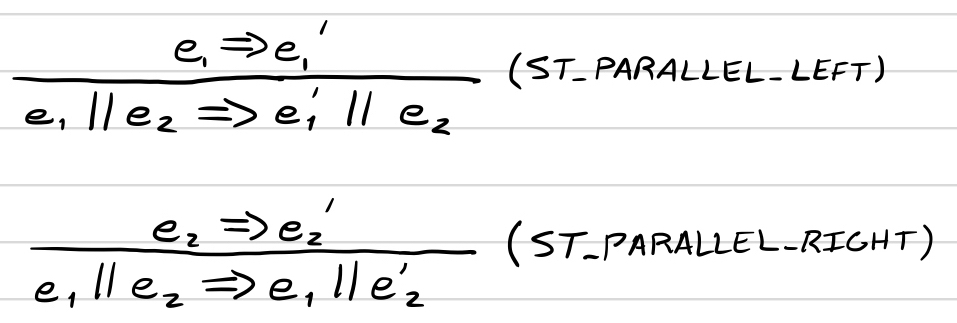
\includegraphics[scale=0.33]{img/ST_PARALLEL.jpeg}
    \caption{Nondeterminism of two MapReduce reduction rules should enable
             semantics to model the uncertain ordering by which concurrent tasks
             are performed.}
  \end{figure}
\end{frame}

\begin{frame}
  \frametitle{Nondeterministic MapReduce Operational Semantics}
  \begin{figure}
    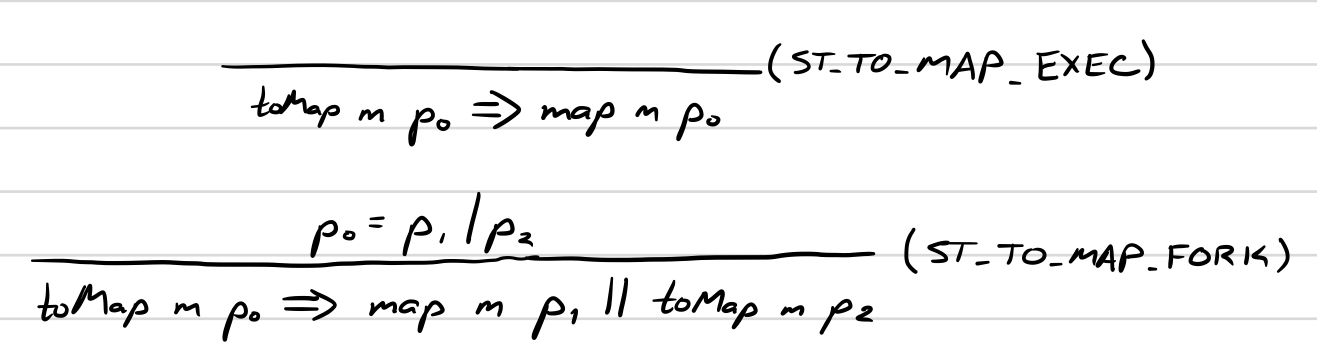
\includegraphics[scale=0.25]{img/ST_TO_MAP.jpeg}
    \caption{Nondeterminism of two MapReduce reduction rules should enable
             semantics to model any number of map task partitions, where each
             task may be given \emph{any} partition of the data.}
  \end{figure}
\end{frame}
